\chapter{関連研究}
関連研究や用語の定義,先行研究及びアプリケーションの先行事例を示す.

\section{時間の定義}
時間管理の定義は表~\ref{tb:Lakein}に示したLakeinの定義\cite{Lakein1989}をはじめとして様々である.

\begin{table}[htb]
\begin{center}
  \begin{tabular}{|l|l|} \hline
   1 & すべきことを決定する \\ \hline
   2 & 達成するための目標を設定する \\ \hline
   3 & 優先順位を決める \\ \hline
   4 & 取り組む課題のプランニングを作る \\ \hline
  \end{tabular}
  \caption{Lakeinによる時間管理の定義}
  \label{tb:Lakein}
\end{center}
\end{table}

Claessens et al. は,先行研究の定義を俯瞰した上で,時間管理を"目標を達成するために時間を効果的に使用する行動"と定義し時間管理の行動を更に以下の3つに分類した\cite{Claessens2007}(表 ~\ref{tb:Claessens}参照).

\begin{table}[htb]
\begin{center}
  \begin{tabular}{|l|l|} \hline
   時間アセスメント行動(time assessment behavior): \\ ~~~過去,現在,未来の時間を認識し,時間の使い方に関して認識する事 \\ \hline
   プランニング行動(planning behavior): \\  ~~~時間を効率的に使用する事を目的とする事 \\ \hline
   モニタリング行動(monitoring behavior): \\ ~~~行動中における時間の配分のモニタリング・不測の事態へのリスクヘッジ等 \\ \hline
  \end{tabular}
  \caption{Claessens et al. による時間管理の定義}
  \label{tb:Claessens}
\end{center}
\end{table}

\section{先行研究について}
時間管理研究は大きく分けて時間管理がもたらす効果の研究と時間管理能力に関する研究の2種類に分けられる.
前者は更に以下の3つに分類が可能である.(表~\ref{tb:senko}参照)
\begin{table}[htb]
\begin{center}
  \begin{tabular}{|l|l|} \hline
   1 & 時間管理と他の指標の相関関係を調べる研究 \\ \hline
   2 & 時間管理のプロセスモデルの研究 \\ \hline
   3 & 時間管理トレーニングの研究 \\ \hline
  \end{tabular}
  \caption{時間管理がもたらす効果の研究の概要}
  \label{tb:senko}
\end{center}
\end{table}

後者の時間管理能力の研究では必要時間の正確な見積もりの能力に関する研究である.
時間管理能力に関しては主に見積もり時間の精度に関して議論されている.
見積もりの精度は大きく分けて課題に対するもの\footnote{与えられた課題の時間 \cite{Roy2008}や経験の有無\cite{Roy2007}}と被験者の個人差によるもの\footnote{時間評価における知覚時間の歪み\cite{Oguro1961}\cite{Murakami2016}}の2種類存在しているが,
原因として記憶との関連性が考えられている\cite{Roy2005}.

正確な見積もりを計算する手法は主に大規模プロジェクト向けに提案される事が多い.
例えばPERT(Program Evaluation and Review Technique)では個々のタスクの見積もりを予測する手法である「三点見積もり法」が考案されている.
タスク完了に要する時間の最良見積もり(期待時間)値を$T_{E}$,タスク完了に必要な最小時間の予測(楽観的時間)を$O$,タスク完了に必要と思われる最頻値の見積時間(最確時間)を$M$,タスク完了に必要な最大時間の予測(悲観的時間)を$P$とすると,下記の様に見積もりを行う.
\[ 
T_{E} = (O + 4M + P) ÷ 6
\] 

\section{日常生活動作、及び個人管理としての時間管理}
日常生活動作(Activities of Daily Living;ADL)とは,人が日常生活において繰り返す,身の回りの活動や動作のことである.具体的には,身の回りの動作(食事,更衣,整容,排泄,入浴の各動作),移動動作,その他生活関連動作(家事動作,交通機関の利用等)を指す\cite{Sakai2003}.
今日では特にパフォーマンスやストレスなど様々な観点から個人管理面においても適切な時間管理が求められている.\cite{Barling1996}\cite{Britton1991}\cite{Burt1994}\cite{Macan1994}.

\section{システムに関して}
今日,日常生活動作を基調とし,身近な時間管理をサポートするシステムが複数開発されている.私は現在開発されたアプリケーションの種類を以下の3種類に分類した.(表 ~\ref{tb:app}参照)

\begin{table}[htb]
\begin{center}
  \begin{tabular}{|l|l|} \hline
   1 & タイムログ \\ \hline
   2 & ルーチン補助 \\ \hline
   3 & ストップウォッチ \\ \hline
  \end{tabular}
  \caption{時間管理ツールの分類}
  \label{tb:app}
\end{center}
\end{table}

1つ目のタイムログに関しては日毎のタスクをなるべく多く記録・計測を行い,一日の時間の使い方を可視化する事を目的としているものである.
このシステムの先行事例には たすくま\cite{Taskuma} や toggl\cite{toggl} (図~\ref{fig:toggl}参照)が挙げられる.
\\
\begin{figure}[ht]
\begin{center}
\begin{tabular}{c}

  	\begin{minipage}[b]{0.5\linewidth}
	\begin{center}
		\fbox{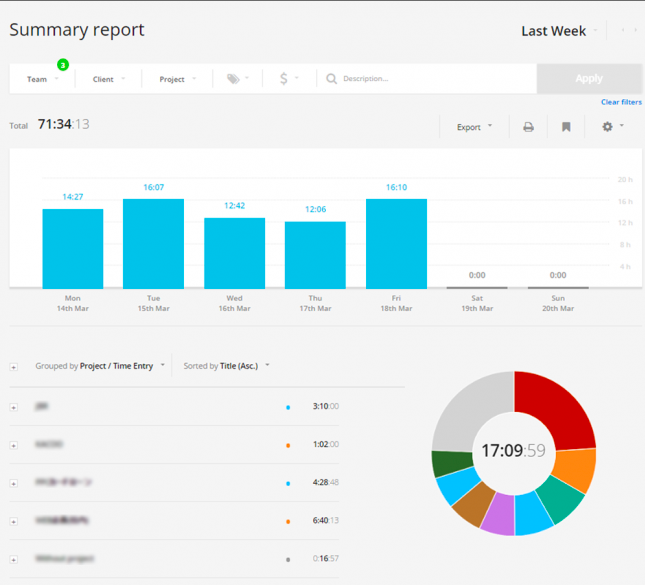
\includegraphics[width=10cm]{images/2/toggl.png}}
		\caption{togglによるログの可視化}
		\label{fig:toggl}
	\end{center}
  	\end{minipage}
\end{tabular}
\end{center}
\end{figure}
\\

2つ目のルーチン補助に関しては,自分がこれから行いたいルーチンをリマインド音などを用いてコントロールするものである.
このシステムの先行事例には自分でやる事を設定する ルーチンタイマー\cite{RoutineTimer} (図~\ref{fig:routine}参照)やポモドーロテクニック\cite{pomodoro} に則ったリマインドアプリなどがある.
\\
\begin{figure}[ht]
\begin{center}
\begin{tabular}{c}

  	\begin{minipage}[b]{0.5\linewidth}
	\begin{center}
		\fbox{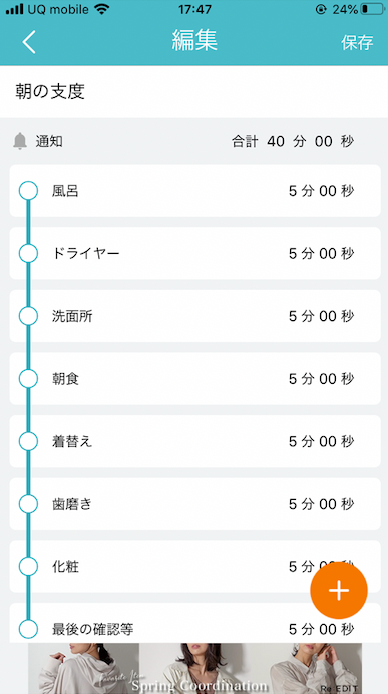
\includegraphics[width=5cm]{images/2/routine.png}}
		\caption{ルーチンタイマーの行動設定例}
		\label{fig:routine}
	\end{center}
  	\end{minipage}
\end{tabular}
\end{center}
\end{figure}
\\
3つ目のストップウォッチに関しては,ストップウォッチを主機能として時間把握に役立てようとするものであり,用途・目的は様々である.
例えば時間の流れをイラストで表現するもの(ねずみタイマー\cite{MouseTimer}(図~\ref{fig:mouse}参照))や時間把握の精度をミニゲームに昇華させたもの\cite{JUSTTIME},ストップウォッチとメモ帳を組み合わせたもの\cite{StopNote}などが挙げられる.
\begin{figure}[ht]
\begin{center}
\begin{tabular}{c}

  	\begin{minipage}[b]{0.5\linewidth}
	\begin{center}
		\fbox{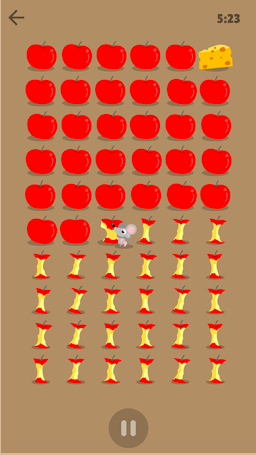
\includegraphics[width=5cm]{images/2/mouse.png}}
		\caption{ねずみタイマーによる経過時間の可視化}
		\label{fig:mouse}
	\end{center}
  	\end{minipage}
\end{tabular}
\end{center}
\end{figure}

\section{まとめ}
本章では,本研究における関連研究を整理し,問題意識を洗い出した.
次章では,筆者が本研究に先立ち行った研究について述べ,問題意識を洗い出す.